\documentclass[a4paper,11pt,twoside,notitlepage]{article}
\usepackage[left=2.5cm,right=2cm,top=2cm,bottom=2cm]{geometry}
\usepackage{graphicx}
\DeclareGraphicsExtensions{.pdf,.jpeg,.jpg}
\usepackage[colorlinks=false, pdfborder={0 0 0}]{hyperref}
\usepackage{cleveref} 
\usepackage{fancyhdr}
\usepackage{abstract}
\usepackage{framed}              %for doing nice boxes
\usepackage{amsmath}             %for math environment
\usepackage{parskip}             %for modifying spacing
\usepackage[procnames]{listings} %for inserting code
\usepackage{color}               %obv
\usepackage{appendix}            %obv
\usepackage{enumitem}            %for modifying lists
\setitemize{noitemsep,topsep=0pt,parsep=0pt,partopsep=0pt}
\setenumerate{noitemsep,topsep=0pt,parsep=0pt,partopsep=0pt}
\usepackage{float}              %for forcefully placing diagrams 
\usepackage[backref=true,
            %style=authoryear,
            style=numeric-comp,
            citereset=section,
            maxcitenames=3,
            maxbibnames=100]{biblatex}
\bibliography{litreview}
\DefineBibliographyStrings{english}{%
    backrefpage  = {see p.}, % for single page number
    backrefpages = {see pp.} % for multiple page numbers
}
\setlength\bibitemsep{1em}
\usepackage{fancyvrb} % for inserting .txt
\usepackage{pgfplots}
\usepackage{caption} % for figures within figures
\usepackage{subcaption} %figures figures
\usepackage{adjustbox}

\usepackage{titlesec}
\titlespacing\section{0pt}{12pt plus 4pt minus 2pt}{0pt plus 2pt minus 2pt}
\titlespacing\subsection{0pt}{12pt plus 4pt minus 2pt}{0pt plus 2pt minus 2pt}
\titlespacing\subsubsection{0pt}{12pt plus 4pt minus 2pt}{0pt plus 2pt minus 2pt}

\usepackage{tikz}
\usetikzlibrary{arrows,chains,matrix,positioning,scopes,calc}
\makeatletter
\tikzset{join/.code=\tikzset{after node path={%
\ifx\tikzchainprevious\pgfutil@empty\else(\tikzchainprevious)%
edge[every join]#1(\tikzchaincurrent)\fi}}}
\makeatother
\tikzset{>=stealth',every on chain/.append style={join},
         every join/.style={->}}
\tikzstyle{labeled}=[execute at begin node=$\scriptstyle,
   execute at end node=$]



        \definecolor{redi}{RGB}{255,38,0}
        \definecolor{yellowi}{RGB}{255,251,0}
        \definecolor{greeni}{RGB}{166,247,166}

        \tikzset{ 
          table/.style={
            matrix of nodes,
            row sep=-\pgflinewidth,
            column sep=-\pgflinewidth,
            nodes={rectangle,draw=black,text width=3ex,align=center},
            text depth=0.5ex,
            text height=2ex,
            nodes in empty cells
          },
          texto/.style={font=\large\sffamily},
          title/.style={font=\large\sffamily}
        }


        \newcommand\CellText[2]{%
          \node[texto,left=of mat#1,anchor=east]
          at (mat#1.west)
          {\large #2};
        }

        \newcommand\SlText[2]{%
          \node[texto,left=of mat#1,anchor=west,rotate=50]
          at ([xshift=1.5ex,yshift=1ex]mat#1.north)
          {\large #2};
        }


\newcommand{\super}[1]{\textsuperscript{#1}}

%% \renewcommand{\cite}[1]{\footcite{#1}}

\definecolor{keywords}{RGB}{255,0,90}
\definecolor{comments}{RGB}{0,0,113}
\definecolor{red}{RGB}{160,0,0}
\definecolor{green}{RGB}{0,150,0}
\lstset{frame=tb,
  language=Python,
  aboveskip=3mm,
  belowskip=3mm,
  showstringspaces=false,
  columns=flexible,
  basicstyle={\small\ttfamily},
  numbers=none,
  numberstyle=\tiny\color{gray},
  keywordstyle=\color{keywords},
  commentstyle=\color{comments},
  stringstyle=\color{red},
  breaklines=true,
  breakatwhitespace=true,
  tabsize=3,
  procnamekeys={def,class}
}

%% %% BOXED ABSTRACT
%% \renewenvironment{abstract}
%%  {
%% 	\small
%%   	\begin{center}
%%   	\bfseries \abstractname\vspace{-.5em}\vspace{0pt}
%%   	\end{center}
%%   	\list{}{
%%     	\setlength{\leftmargin}{.5cm}%
%%     	\setlength{\rightmargin}{\leftmargin}%
%%   	}%
%%   	\item\relax}
%%  	{\endlist}

%% OK LETS GO I GUESS
\begin{document}
	\title{Copyright Model for Collaboration
		\\ \small Literature Review}
	\author{William Marsey
		\\Imperial College London}
	\date{June 2014}
 	\maketitle	
        
        \tableofcontents

        \clearpage
        %%%%%%%%%%%%%%%%%%%%%%%%%%%%%%%%%%%%%%%%%%%%%%%%%%%%%%%%%%%%
        %%
        %% THE QUESTION --- COMPLETE REWRITE PLEASE
        %%
        %%%%%%%%%%%%%%%%%%%%%%%%%%%%%%%%%%%%%%%%%%%%%%%%%%%%%%%%%%%%

        \section{Introduction}
        This project will endeavor to evaluate individual
        contribution in the context of large-scale online
        collaboration. Given a collaboratively edited document, and
        information about each edit of which that article is
        consequent, may we define each collaborator in terms of their
        stake in the document? How do we algorithmically define the
        value of a contribution in this context?

        Taking a Wikipedia article and its revision history, this
        project aims to assign each editor a weighted value, according
        to the algorithmic analysis of the version
        generated by each edit. One of the main aims of this project is to produce
        a system that will allow for a visualisation of the
        distribution of this `wealth' amongst the users.
        
        In this literature review we begin with a brief overview of
        the concept of edit distance, including the various algorithms
        that have been devised in order to measure it. We then give an
        overview of existing research into Wikipedia revision
        histories that leverage these algorithms. We conclude with a
        general overview of the goals of this project, including the
        metrics by which we will measure contribution.

       %%%%%%%%%%%%%%%%%%%%%%%%%%%%%%%%%%%%%%%%%%%%%%%%%%%%%%%%%%%%
       %%
       %% EDIT DIFFERENCE
       %%
       %%%%%%%%%%%%%%%%%%%%%%%%%%%%%%%%%%%%%%%%%%%%%%%%%%%%%%%%%%%%
        \section{Previous work}
        \subsection{Edit difference algorithms}
        To measure difference between different text revisions, we
        will refer edit distance. Edit distance between two texts,
        as first defined in the research of Levenshtein,\cite{Levenshtein1966} can be defined as the minimum
        amount of insert, delete and substitutions operations needed
        to transform one text into another.

        \begin{figure}[h]
          \centering
                  
          \begin{tikzpicture}[node distance =3pt and 0.5cm,anchor=center]
                    
            \matrix[table] (mat11) { |[fill=greeni]| &
              |[fill=yellowi]|F & O & R & K & |[fill=redi]|S
              \\ |[fill=greeni]|S & |[fill=yellowi]|P & O & R & K &
              |[fill=redi]| \\ };

            \CellText{11-1-1}{string 1:}; \CellText{11-2-1}{string
              2:};

            \SlText{11-1-1}{Insert} \SlText{11-1-2}{Swap}
            \SlText{11-1-6}{Delete}
            
          \end{tikzpicture}

          \vspace{3 mm}

          forks $\rightarrow$ spork, edit distance: 3
          
          \caption{An edit distance example using all three
            operations}
          \label{fig:fork-spork}
        \end{figure}

        Levenshtein's characterisation of this distance is given as:
        
        \begin{figure}[H]
          \centering
          for the function $\mbox{lev}_{a,b}(|a|,|b|)$:\\
          $$\mbox{lev}_{a,b}(i,j) = 
             \left\{
                \begin{array}{ll}
                  \mbox{max}(i,j) & \mbox{if }min(i,j) = 0\\
                  \mbox{min}\left\{
                        \begin{array}{lll}
                          lev_{a,b}(i-1,j)+1\\
                          lev_{a,b}(i,j-1)+1\\
                          lev_{a,b}(i-1,j-1)+1_{(a_i{\neq}b_j)}
                        \end{array}
                      \right.
	                & else 
	        \end{array}
             \right.$$
             when $a_i = b_j$, $1_{(a_i{\neq}b_j)} = 1$\\
             when  $a_i \neq b_j$, $1_{(a_i{\neq}b_j)} = 0$
        \end{figure}

        That is, the distance between two strings is characterised the
        minimum distance between three different pair-combinations of its
        substrings. A 'text-book' implementation of this algorithm can
        be represented by the pseudo-code below. (We present the
        dynamic-programming-style algorithm here, and will generally
        be working with dynamic programming implementations throughout
        the study.)
        
        \begin{figure}[H]
          \centering
          \begin{lstlisting}
          ed(x,y):
             #end base cases
             if |x| = 0: return |y|
             if |y| = 0: return |x|    

             #end table initialisation
             d is a table [0..|x|][0..|y|]
             for i = 1 to |m|:
                 d[i,0] = i
             for j = 0 to |y|:
                 d[0,j] = j           
             
             #dynamic computation
             for j = 1 to |y|:
                 for i = 1 to |x|:
                     c = [(x[i] == y[j]) ? O else 1]
                     ins = d[i-1,j] + 1
                     dlt =d[i,j-1] + 1
                     kp_swp = d[i-1,j-1] + c
                     d[i,j] = min(ins, dlt, kp-swp)
             
             #return last computed number
             return d[|x|,|y|]
        \end{lstlisting}
        \caption{Basic dynamic implementation of Levenshtein distance}
        \label{fig:levenshtein-dynamic}
        \end{figure}

        We can see that on comparing strings $x$ and $y$, a $|x|$ by
        $|y|$ table is created, and then filled with values. For this
        reason both the time and space complexity of the algorithm is
        $\theta (|x||y|)$.

        Reducing the space needed for this computation is relatively
        easy, and can be done in a few different ways. One way is to
        simply disregard parts of the table already computed. We can
        see that, on each computation of $d[i,j]$ (as it appears
        above), we require only a small part of the matrix:
        $d[i-1,j-1]$, $d[i-1,j]$ and $d[i,j-1]$. At any iteration $i$,
        where is great than $1$, we may disregard rows $0 \dots (i-2)$
        inclusive.

        There are more complicated techniques that allow us to also disregard
        unneccesary computation --- a few implementations employ
        strategies that allow them to trace the table space
        diagonally, rather than iteratively, achieving a
        time complexities as low as $O(ed(x, y)^2)$.\cite{Chang1992}
        Another harnesses bit vectors to achieve a time complexity of
        $O(nm/w)$ or $O(nm log {\Sigma}/w)$ time where $w$ the
        bit-word size of the machine, and $\Sigma$ is the alphabet
        size.\cite{Myers1999}\cite{Hyyro2003} These optimisations will
        be explored in this project.

        \subsubsection*{Varieties of edit distance}
        Modifications can be made to the nature of the distance
        itself, in order to adapt the measure a variety of different and
        specific needs. Here is a brief overview of the main groups
        these extensions fall into:

        \begin{itemize}
          \item \textbf{Hamming distance.} This allows for
            substitutions only, comparing same-length strings, such
            that:\\ 
            $ed_{hamming}(\text{``abc''},\text{``abd''}) =1$,\\ 
            $ed_{hamming}(\text{``abc''},\text{``bcd''}) = 3$,\\ 
            and $ed_{hamming}(\text{``abc''},\text{``ab''})$ is
            undefined.\cite{Hamming1950}
          \item \textbf{Reversals.} The Damerau-Levenshtein distance
            defines an `swap' operation, which is the reversal of two
            adjacent characters. It is particularly suited to
            spell-checking, and for analysing DNA-sequence
            variations. In this case:\\ 
            $ed_{damerau}(\text{``ab''},\text{``ba''}) = 1$
          \item \textbf{Block distance.} This allows for displacements
            of entire blocks to count as one operation. For example:\\
            $ed_{block}(\text{``abcde''},\text{``cdeax''})= 2$ \\
            One move of the block `cde', one substitution of `b'
            for `x'.\cite{Tichy1984}
          \item \textbf{\textit{q}-grams distance.} \textit{q}-grams
            are simply sub-strings, and this measure describes the
            similarity of two strings in terms of \textit{q}-grams
            they share.\cite{Ukkonen1992}\\
            $ed_{q-gram}(x,y)=\sum\limits_{v\in\Sigma ^q}|G(x)[v]-G(y)[v]|$\\ 
            where $G(x)[v]$ returns the number of occurrences of
            \textit{q}-gram v in string x, and $\Sigma ^q$ is all the
            possible \textit{q}-grams in the
            alphabet (capped by string length). $|G(x)[v]-G(y)[v]|$ a
            large positive number every time a \textit{q}-gram appears
            a large amount of times in one string, but not the other;
            it returns 0 if the substring apears the same number of
            times. So, the whole function measures this difference for
            all possible substrings, and sums them, returning a high
            number for difference, and a low number for similarity.
        \end{itemize}

        Other algorithms we may look at are those that, like the
        \textit{q}-gram distance, principally concern themselves with
        finding common subsequences between the strings. The common
        subsequence problem relates to the edit distance problem by
        way of the heuristic that two similar strings will have
        similar subsequences --- the \textit{q}-gram algorithm, for
        instance, relies on this heuristic, and works well for most
        texts, it does not agree with all distance measures. For
        example, two strings that are very different according to this
        heuristic may be quite similar according to the
        Damrau-Levenshtein measure.
        
        \subsubsection*{Optimal alignment}
        Another part of the problem of working out optimal edit
        distance is finding the `optimal alignment' --- the measures
        are closely related. We displace and arrange the characters of
        a string such that the set of operations to transform each
        character into its counterpart is minimal. For example, in
        figure \ref{fig:fork-spork}, the alignment of the two strings
        ``fork'' and ``spork'' was:

        \begin{center}
          \begin{tabular}{cccccc}
            s & p & o & r & k & -\\
            - & f & o & r & k & s 
          \end{tabular}
        \end{center}

        However it could also conceivably have been:

        \begin{center}
          \begin{tabular}{ccccccccccccccccc}
            s & p & o & r & k & - & & or even & & - & s & p & o & - & r & k &\\
            f & - & o & r & k & s & &         & & f & - & o & - & r & k & - & s    
          \end{tabular}
        \end{center}

        Here, the left-hand version results in an equivalent
        Levenshtein distance, but we can see how the distance for the
        right-hand example would be sub-optimal.

        \begin{figure}[h]
          \centering   
          \begin{tikzpicture}[node distance =3pt and 0.5cm,anchor=center]
            \matrix[table] (mat11) {|[fill=greeni]|  & |[fill=redi]|S & |[fill=yellowi]|P & |[fill=redi]|O & |[fill=greeni]|  & |[fill=redi]|R & K & |[fill=greeni]|\\
                                    |[fill=greeni]|F & |[fill=redi]|  & |[fill=yellowi]|O & |[fill=redi]|  & |[fill=greeni]|R & |[fill=redi]|  & K & |[fill=greeni]|S\\};
            
            \CellText{11-1-1}{string 1:}; \CellText{11-2-1}{string
              2:};

            \SlText{11-1-1}{Insert}
            \SlText{11-1-2}{Delete}
            \SlText{11-1-3}{Swap}
            \SlText{11-1-4}{Delete}
            \SlText{11-1-5}{Insert}
            \SlText{11-1-6}{Delete}
            \SlText{11-1-8}{Insert}
          \end{tikzpicture}\\
          \vspace{3 mm}
          spork $\rightarrow$ forks, edit distance: 7
          \caption{An sub-optimal edit distance example}
          \label{fig:fork-spork-subopt}
        \end{figure}

        The Smith-Waterman algorithm calculates optimal alignment by
        populating two tables --- one like that in the pseudocode
        above, and also as a table of arrows. These arrows define a
        path from one corner of the table space to the other. The
        shape of this path defines how to align the two
        strings.\cite{Smith1981} See figure
        \ref{fig:smith-waterman-traceback} for an example.

        This path may also be read as an edit operation. An arrow at
        the position $[i,j]$ in the table defines edit operations for
        $x[i]$ and/or $y[j]$ thus:
        \begin{itemize}
          \item \textbf{$\nwarrow$ at $[i,j]$, if $x[i] \neq y[j]$}
            \\ Denotes a 'swap' between $x[i]$ and $y[j]$ (if $x[i] =
            y[j]$ then it denotes the lack of an operation).
          \item \textbf{$\uparrow$ at $[i,j]$}\\Denotes the deletion
            of $x[i]$
          \item \textbf{$\leftarrow$ at $[i,j]$}\\Denotes the
            insertion of $y[j]$
        \end{itemize}
        
        \begin{figure}[h]
          \centering
          $\left\{
                \begin{array}{ccccccc}
                    &   & S & P & O & R & K \\
                    & \color{red}{0} & \color{red}{0} & 0 & 0 & 0 & 0 \\
                  F & 0 & \nwarrow & \color{red}{\nwarrow} & \nwarrow & \nwarrow & \nwarrow \\
                  O & 0 & \uparrow & \nwarrow & \color{red}{\nwarrow} & \downarrow & \leftarrow \\
                  R & 0 & \uparrow & \uparrow & \uparrow & \color{red}{\nwarrow} & \leftarrow \\
                  K & 0 & \uparrow & \uparrow & \uparrow & \uparrow & \color{red}{\nwarrow} \\
                  S & 0 & \nwarrow & \uparrow & \uparrow & \uparrow & \color{red}{\uparrow} \\
                \end{array}\right\} $\\
                (If the arrow reaches an edge before the left-hand
                corner, we trace along that edge, reading each shift
                as an arrow in the direction of the trace.)
                \caption{Diagram showing Smith-Waterman traceback path
                  (in red) on the edit operation forks $\rightarrow$
                  spork}
          \label{fig:smith-waterman-traceback}
        \end{figure}

        \subsubsection*{Delta encoding}
        Finally, we may also look into Delta encoding
        algorithms. These describe ways of compressing the storage of
        a document's history --- a format in which only the
        differences between each text is stored, not the entire
        version. These algorithms are of the same family of algorithms
        discussed above. In fact, we find that one of the fastest
        known algorithms,\footnote{According to Hunt's 1998
          study\cite{Hunt1998}} \textit{VDelta}, is a refinement of
        the block distance algorithm mentioned above. For a given
        version $n$ of a document $doc$ is defined as:
        
        $$v_n = v_0 \cup {\Delta}(v_0,v_1) \cup {\Delta}(v_1,v_2)
        \cup \dots \cup {\Delta}(v_{n-1},v_n) $$

        where ${\Delta}(v_i,v_j)$ is the difference between version
        $i$ and version $j$ of the document, and the union operation
        $\cup$ combines each version in a manner particular to the
        $\Delta$ data-type. Storing data in this way can be very
        efficient, resulting in a compression factors of five or ten
        on typical data.\cite{Macdonald2000} It may also be relatively
        easy to maintain in our case, due to the linear nature of
        Wikipedia revision histories.

       %%%%%%%%%%%%%%%%%%%%%%%%%%%%%%%%%%%%%%%%%%%%%%%%%%%%%%%%%%%%
       %%
       %% WIKIPEDIA
       %%
       %%%%%%%%%%%%%%%%%%%%%%%%%%%%%%%%%%%%%%%%%%%%%%%%%%%%%%%%%%%%
        \subsection{Wikipedia}
        \subsubsection*{In academia}
        Wikipedia is a free, open-source, publicly-editable online
        knowledge-base. The software is runs upon, MediaWiki, is also
        open-source, powering countless other online
        encyclopedias. Since it's launch in 2001, Wikipedia has become
        a the pre-eminent online source of reference. The website is
        ranked 6\super{th} globally in terms of website traffic, and
        is the highest-ranked reference website by far - most of the
        sites it shares the top spots with are portals, search
        engines, shopping mega-sites, and social media
        websites.\footnote{According to `Alexa', an website ranking
          company.\cite{Alexa-about2014} Though, this may be an
          underestimation. Alexa may well be biased towards English
          speakers and Internet Explorer users, underestimating
          Wikipedia.org's popularity, since `two thirds of all
          Wikipedia articles are in languages other than
          English'\cite{wikimedia-noteonalexa}} Despite early
        skepticism (particularly concern over the inherent chaos in
        the system: ``...edits, contributed in a predominantly
        undirected and haphazard fashion by ... unvetted
        volunteers.''\cite{Wilkinson2007}), it is widely claimed to be
        a success, `the best-developed attempt thus far of the
        enduring quest to gather all human knowledge in one
        place'\cite{Mesgari2014}.

        That Wikipedia has become a hub of research in many fields is
        also self-evident to anyone who has searched for articles on
        the subject. Mesgari et al, just quoted, has prepared a very
        recent `systematic review of scholarly research on the content
        of Wikipedia', which gives an overview of 110 articles on the
        subject --- attesting to his observation that Wikipedia
        has been `irresistable point of unquiry for researchers from
        various fields of knowledge'. It will be a useful touching
        stone for this study, finding 82 out of the 110 surveyed
        articles to concern Wikipedia quality. Some of these are also
        referenced here, and many of the others will come to bear on
        the study as it progresses.

        Other important general sources will be WikiLit,\cite{wikilit}
        AcaWiki\cite{acawiki} and WikiPapers\cite{wikipapers}, all of
        which are online repositories of academic research into
        Wikipedia and other Wikis.       

        %%%%%%%%%%%%%%%%%%%%%%%%%%%%%%%%%%%%%%%%%%%%%%%%%%%%%%%%%%%%
        %%
        %% WIKIPEDIA ARTICLE QUALITY
        %%
        %%%%%%%%%%%%%%%%%%%%%%%%%%%%%%%%%%%%%%%%%%%%%%%%%%%%%%%%%%%%
        
        \subsubsection*{Studies of Wikipedia revision history}
        Tangentialy related studies fall into two major groups: studies
        of Wikipedia article quality and studies of edit behaviour.
        It is from the first group that we find the most pertinent
        work --- it is also one of the most fruitful areas of
        research.

        It is the metrics used to measure quality in these studies
        that are of most use to us here. We don't concern ourselves
        with the quality of the article on the whole, but many studies
        have endeavoured to find out what kind of article content can
        be automatically recognised. High numbers of Links, internal
        links, images and formulas have been found to indicate
        percieved quality,\cite{Lucassen2010}\cite{mcguinness2006} and
        these are easy to identify using Wikipedia's markup
        language. Other useful meterics have been the age of the
        word,\cite{Cross2006} the age and rate of change of the
        article in comparison to other articles,\cite{Zeng2006} and
        the recent activity of the article (an article undergoing a
        peak in edit changes may be `unstable').\cite{Adler2006}
        Another study of particular interest is that of Stvilia et al,
        which found metrics of article quality through factor
        analysis,\cite{Stvilia2005} confirming much of the ideas
        already mentioned.

        A landmark piece of work is the Wikitrust
        software.\cite{Adler2007} Wikitrust was\footnote{Defunct as of
          author's checks, Apr 2014} a firefox plugin, designed to
        highlight the words of a Wikipedia article with different
        colors. The gradations of these colors relate to levels of
        trust, and the computations made to derive them were based
        upon the metrics mentioned above, with particular emphasis on
        a word's age. A screenshot can be seen in figure
        \ref{fig:wikitrust}. The program was reviewed as recently as
        2011,\cite{Lucassen2011} and it was found to be basically flawed,
        with users not really seeing the use for it (it was found
        that, having read Wikipedia before, they already had a good
        idea of how to rate an article). However, the Wikitrust team's
        implementation of the quality measures described above will
        prove to be very useful study.
        
       \begin{figure}
         \centering
         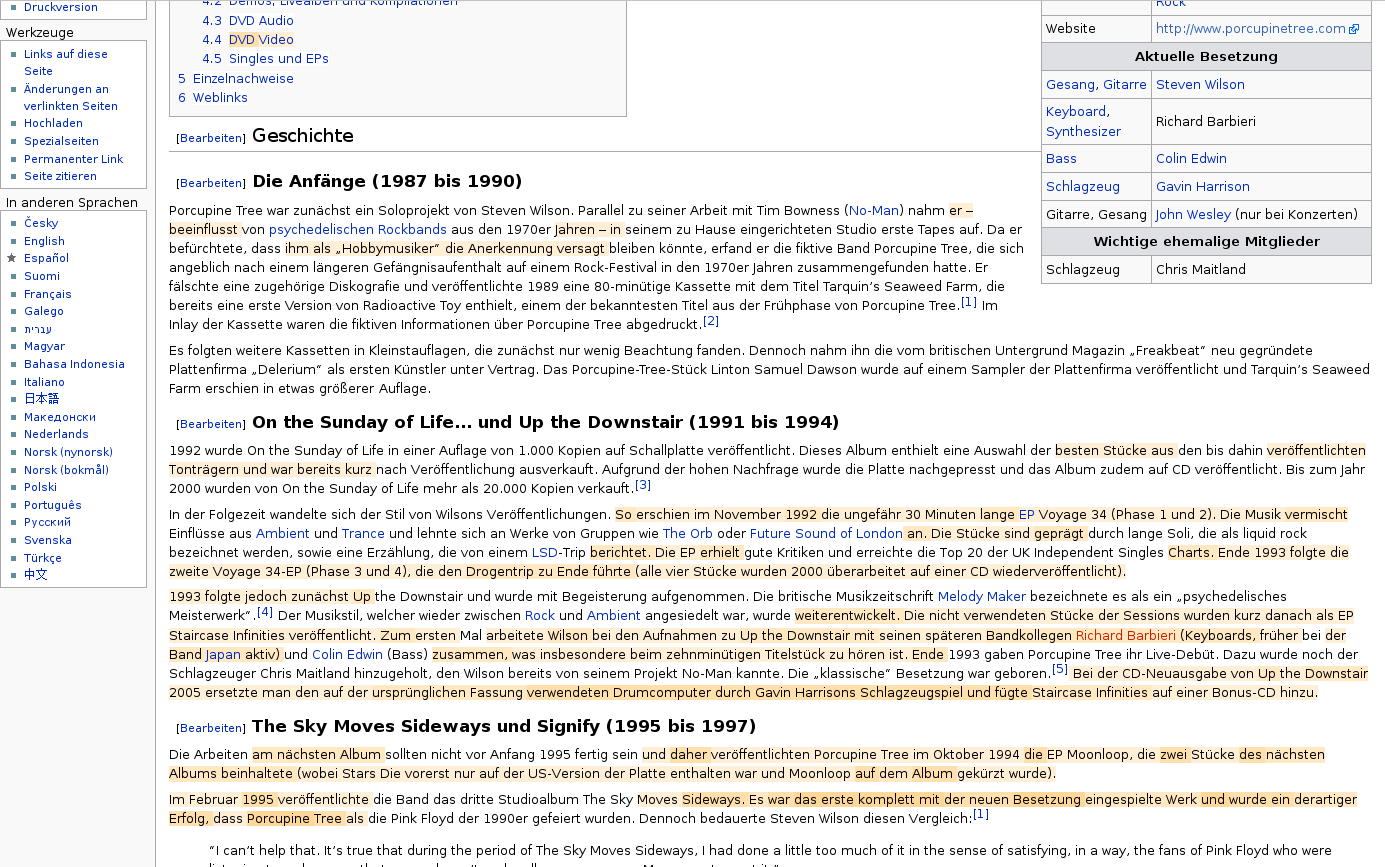
\includegraphics[width=0.8\textwidth,clip=true,resolution=300]{img/wikitrust.png}
         \caption{Wikitrust in action, 2011}
         \label{fig:wikitrust}
       \end{figure}

        Another metric which may also affect the quality of an article as
        a resource, is logical structure. It was found in 2005 that
        this, if anything, was the clearest difference between
        Wikipedia and commercial encyclopedias,\cite{Giles2005}
        supporting previous conjecture.\cite{Denning2005} Not many
        studies have concerned themselves with structure, but later we
        will discuss how we may automatically recognise structural
        change.
        
        A few other key studies present us with useful analyses of
        edit behaviour. Analyses of conflict between authors shows the
        possible reversion cases we will have to recognise. They
        reveal the high number of immediate `undo'-type revisions, and
        also that malicious or unnecessary input may survive several
        versions before being undone. Some study these conflicts as a
        characterisation of normal editing
        behaviour,\cite{Kittur2007}\cite{Kittur2009}\cite{Kittur2010}\cite{Potthast2008}
        while others look to controversial articles,\cite{Iba2010} or
        articles recently cited in the press.\cite{Lih2004} We find
        from these same studies that articles lead by small groups of
        `leaders' produce articles of better quality than those with a
        more homogeneous contribution group, that a small group of
        editors contribute to most of Wikipedia, and that conflict and
        bureaucracy (increasing over time) are the major limiting
        factors in the growth of an article.\cite{Suh2009} Knowledge
        of this context is vital in evaluating the edits we will
        eventually analyse.

        %%%%%%%%%%%%%%%%%%%%%%%%%%%%%%%%%%%%%%%%%%%%%%%%%%%%%%%%%%%%
        %%
        %% CONCLUSIONS
        %%
        %%%%%%%%%%%%%%%%%%%%%%%%%%%%%%%%%%%%%%%%%%%%%%%%%%%%%%%%%%%%

        \section{Conclusions}
        Now we have reviewed the existing work, we will begin to
        outline our intentions for the design of our own algorithm. Here
        we discuss the assumptions that we make about our data, our
        intentions with regards to analysing that data, and the
        metrics by which we will regard each contribution.

        %% ASSUMPTIONS
        \subsubsection*{Assumptions}
        \begin{itemize}
          \item \textbf{We assume that the final, or `target' article
            is of `good' quality.} There are many studies which concern
            themselves with verifying the accuracy and quality of
            Wikipedia articles --- In this study we are specifically
            concerned with the quality of contribution, i.e. the
            quality of text within the article, relative to the domain
            of the article. Here, the quality of the article itself is a
            moot point.
          \item \textbf{We assume the article is well-formed.} As much
            as we do not concern ourselves with article accuracy, we
            also assume that the Wikipedia markup is also
            well-formed. We may also eventually check whether links
            are invalid, but for the moment we assume that they are.
          \item \textbf{We make no distinction between humans, bots
            and anonymous editors.}
        \end{itemize}
        
        %%WEIGHTING BY MARKUP
        \subsubsection*{Weighting contribution by markup}
        Given the extensive research regarding which features of a
        wikipedia article are most important, we may define the
        following features to have more weight than standard text from
        the outset:
        \begin{itemize}
          \item Links
          \item Images
          \item Equations
        \end{itemize}

        We may either preprocess the text to identify the each of
        these different `flavours' of input by their Wikipedia mark-up
        conventions, or we may be able to more fluently work them into
        the main difference algorithm, raising and lowering flags
        during runtime.

        %%RESTRUCTURING
        \subsubsection*{Awarding restructuring}
        \label{restructuring}
        It has been found that, even in the most accurate articles,
        that the structure of Wikipedia article can be
        weak.\cite{Giles2005} We should award attempts to reorganize
        articles, possibly looking out for lange block displacements.
        
        %%DENSITY
        \subsubsection*{Awarding the dense edits}
        We should give extra reward to the density of the
        changes. Perhaps we can propose the heuristic: A denser edit
        means more significant change. If we have a set
        of the indexes of an edit operation as
        $\{op_0,op_1,op_2,\dots, op_n\}$, where $op_i$ is the index of
        the $i$th operation, then we may evaluate it's density with a
        standard deviation of the edit itself, $\sigma_{ed}$,
        multiplied by the span of the edit itself in context of the
        wider article, and some weighting factor k. Something along
        the lines of:
        $$ed_{density} = k\bullet\frac{(op_n -
          op_0)\sigma_{ed}}{|v_{ed}|}$$ where $|v_{ed}|$ is the overall
        length of resultant version. By implementing this carefully,
        we may achieve a gradient of weighting, with a lower weight
        values for things like spell-checks, and higher values for
        whole-paragraph changes.

        \subsection*{Undone and partially undone operations}
        We consider three different ways of classifying an edit as
        valueless, or partially valueless. Two ways of classifying
        these kinds of edit are found in previous research, and are
        covered in figure \ref{fig:undo}.

        \begin{figure}[h]
          \centering
          \begin{tikzpicture}
            \matrix (m) [matrix of math nodes, row sep=4em, column
              sep=4em]{ & v_i & \\ v_{i-1} & & v_{i+1}\\ };
            \path[-stealth] (m-2-1) edge node [left]
                 {$ed(v_{i-1},v_i)$} (m-1-2) edge node [below]
                 {$ed(v_{i-1},v_{i+1})$} (m-2-3) (m-1-2) edge node
                 [right] {$ed(v_i,v_{i+1})$} (m-2-3); 
          \end{tikzpicture}\\
          \textit{case a)} if $ed(v_{i-1},v_i) < ed(v_{i-1},v_i) +
          ed(v_{i},v_{i+1})$, then $ed(v_{i-1},v_i)$ has been
          partially undone.\\ 
          \textit{case b)} if $ed(v_{i-1},v_{i+1}) = 0$
          ($v_{i-1} = v_{i+1}$), then $ed(v_{i-1},v_i)$ has been
          completely undone.
          \caption{Diagram showing identification of a partially or
            completely undone edit}
          \label{fig:undo}
        \end{figure}

        Figure \ref{fig:undo} shows how we may identify undone or
        partially undone edits, when they are undone immediately, as
        layed out in Adler et al.\cite{Adler2007} The triangle
        represents three consecutive revisions, and the arrows are the
        edit operations that transform one to another. By calculating
        the edit distance between the distance versions $v_{i-1}$ and
        $v_{i+1}$ we may characterise a longer history of revisions
        than usual, and use that context in order to re-characterise
        the edits it encompasses. In the figure above, case $a$
        describes $v_i$ as a 'diversion'. If $v_{i-1}$ can be
        transformed into $v_{i+1}$ with less operations than the two
        edits that actually bridged that gap, then perhaps some of the
        edits in $v_{i-1} \rightarrow v_i$ were unnecessary, and
        undone by $v_{i+1}$. In this case, we may punish the edit
        $v_{i-1} \rightarrow v_i$ (for the diversion), reward $v_{i}
        \rightarrow v_{i+1}$, or both. Case $b$ is an extreme version
        of $a$ --- the texts $v_{i-1}$ and $v_{i+1}$ are identical, so
        the changes in $v_i$ must have been completely undone. These
        reverts are common in normal Wikipedia edit
        practice.\cite{wiki-revert}

        This algorithm, however, is limited in its scope, and we may
        come across situations where reversions occur over a series of
        edits. Although the system may easily be extended to cover
        larger spans of history, to consider many nodes would require
        the edit-distance computation of very many different node
        pairs. 

        Let us propose a more efficient way of characterising
        redundant entries in terms of longer history spans. We must
        utilise the fact that we have take one article to be the
        ultimate destination of all previous edits in order to do
        so. Let us graph the entirety of a wikipedia's revision
        history in terms of the edit distance from this final version,
        thus:

        \begin{center}
          \pgfplotsset{width=0.4\textwidth}
          \begin{tikzpicture}
            \begin{axis}[
                title={Dummy revision history},
                ylabel={Ed. distance from final},
                xlabel={revision ID},
              ]
              \addplot table {dat/dummy_history.dat};
            \end{axis}
          \end{tikzpicture}
          \label{fig:dummy_history}
        \end{center}
        
        Each point represents a different version, and each line
        represents the the edit-distance between each version. Given
        this information, we may consider only those revisions that
        bring us closer to the final version. They appear on this
        graph as lines with a negative gradient (blue); those with a
        positive gradient take us further away from the final version
        (red):

          \begin{center}
          \pgfplotsset{width=0.4\textwidth}
          \begin{tikzpicture}
            \begin{axis}[
                title={Dummy revision history},
                ylabel={Ed. distance from final},
                xlabel={revision ID},
              ]
              \addplot [blue] table {dat/dummy1.dat};
              \addplot [red] table {dat/dummy2.dat};
              \addplot [blue] table {dat/dummy3.dat};
              \addplot [blue, only marks] table {dat/dummy4.dat};
            \end{axis}
          \end{tikzpicture}
          \end{center}

        We need not computer edit distances with a positive gradient
        (the two red lines). This is simple to implement. Given a
        version $v_i$, having computed it's immediate edit distance
        $ed(v_{i-1},v_i)$, and it's edit distance from the final
        version, $ed_{final_i}$, we know our next computation must be
        $ed(v_{j-1},ed_j)$, such that $j$ is the smallest number that
        satisfies the qualities $j > i$ and $ed_{final_j} <
        ed_{final_{j-1}}$.

        Another possible strategy would be to disregard all edit
        distances that, at any point, lie between two versions that
        are further away from final version than the version
        currently being considered.

          \begin{center}
          \pgfplotsset{width=0.4\textwidth}
          \begin{tikzpicture}
            \begin{axis}[
                title={Dummy revision history},
                ylabel={Ed. distance from final},
                xlabel={revision ID},
              ]
              \addplot [blue] table {dat/dummy1.dat};
              \addplot [red] table {dat/dummy5.dat};
              \addplot [blue] table {dat/dummy6.dat};
              \addplot [blue, only marks] table {dat/dummy4.dat};
              \fill [green!25,fill opacity=0.5] (axis cs:4,13) rectangle (rel axis
              cs:1,0);
              \addplot[red,dashed,update limits=false] 
	      coordinates {(-2,13) (14,13)};
              \addplot[red,dashed,update limits=false] 
	      coordinates {(4,-2) (4,23)};
            \end{axis}
          \end{tikzpicture}
          \end{center}
        
        In this graph, $v_i$, the currently considered version, is
        represented by the node at (4,13). The green rectangle shows
        the area in which we look to find $v_j$, and the blue lines
        are those edit distances we both to compute. In this case,
        after considering $v_i$, we move to the $v_j$ such that $j$ is
        the smallest number that satisfies to qualities $j > i$ and
        $ed_{final_j} < ed_{final_i}$. In this graph above we move
        from (4,13) to (8,12).

        It is worth stating here that, in both these strategies, after
        discovering $v_j$, we always compute $ed(v_{j-1}, v_j)$ rather
        than $ed(v_i,v_j)$. We will look into the pros and cons of
        these different strategies further into the project.

        \subsection*{Possible extensions}
        \subsubsection*{Visualisation}
        Given that we are distributing wealth according to a series of
        weight factors, it may be useful to devise a system that
        visualises how these weight factors affect distribution. This
        would simplybe a matter of expressing the final
        `score' in terms of these variables, and producing some
        interactive graphs. Several good attempts have been made to
        visualise Wikipedia history data, with varying levels of
        success,\cite{Chi2008}\cite{Sabel2007}\cite{Suh2007}\cite{Wu2013}\cite{Viegas2004} so the
        work would be well supported. We will look into the viability
        of this extension further into the project.
        
        \subsubsection*{Extending data}
        Current intentions are to approach the data on an
        article-by-article basis, grabbing a particular version and
        tracing its history backwards. We grab the pages using HTTP
        requests, via Mediawiki's inbuilt API. We could, however,
        download Wikipedia in its entirety. The entire site is
        compressed and dumped monthly, and the dumps are free to
        download (though they are 800GB compressed).\cite{wiki-dump}

        \subsubsection*{Further analysis}
        Given the over-arching nature of Wikis, it may be possible to
        derive other information about the articles we
        study. Past studies have used revision histories in order to
        figure out a variety of different things, including a
        2012 study which used it to predict box-office
        success,\cite{Mestyan2012} a 2009 study that was able to
        geo-locate editors by their edits.\cite{Lieberman2009}

        Given the by-products of our study, we may be able compare and
        contrast different categories of article, or editor. It would
        be interesting to contrast the actions of humans, and
        bots,\footnote{It has been noted that there are around 700
          bots registered on Wikipedia (as of 2014). Though not all of
          them make edits, those that do are very prolific, and are
          known to reverse malicious submisions in a matter of
          seconds.\cite{wiki-bots}\cite{bbc-bots}} and perhaps look at
        the nature of edits made by different groups of editors.

        \subsubsection*{Further subjects}
        The project may well extend to subjects beyond Wikipedia. A
        git project history, for instance, may be of interest for
        further study. We may combine the existing research with
        metrics that concern code in particular,
        such as Cyclomatic Complexity, which measures code flow
        complexity according to its logical
        operators.\cite{McCabe1976} It would also be interesting to
        figure out a way of changing our algorithm in order to regard
        non-linear revision histories.

        \section{Progress report}
        So far I have written two Python classes, which, together
        can fetch an entire history of a wikipedia article, and
        compute Levenshtein distances between the texts.

        WikiRevisionScrape is a Python class which harnesses the
        Wikipedia API in order to download various pieces of
        information about articles and their histories. It is inspired
        by open Wikipedia metadata classes such as 'Wikipedia
        Miner'\cite{wiki-miner}, or the revision-fetching 'Java
        Wikipedia Library / Wikipedia Revision
        Library'.\cite{wiki-java}\cite{Ferschke2011}

        If the user doesn't specify a particular article title, we
        choose a random one, and trace it's history back. We can also
        set a parameter in order to pick a random article multiple
        times. There are various ways of improving the efficiency of
        this program (such as requesting multiple pages at once), and
        this will be introduced in a later version. At the moment the
        scraper is fully functional, though at the moment saves the data
        in CSV files. I will change this so that it uses a postgres
        database. \textbf{Code and example output can be found in appendix
        \ref{wiki-scrape} starting page \pageref{wiki-scrape}.}

        Another python class, LevDistBasic, is a naive implementation
        of Levenshtein distance (no space or speed
        optimisations). It is a first-attempt implementation of the
        algorithm, and it can return the Levenshtein distance, the
        computation table, the edit operation (in two different
        formats --- human readable, and as a list of tuples). Future
        changes are many, such as including weightings for different
        kinds of string, more space-efficient and speed efficient
        implementations, etc. \textbf{Code and example output can be found in
        appendix \ref{levenshtein-implement} starting page
        \pageref{levenshtein-implement}.}

        These two classes can be entwined manually, by fetching two
        pieces of data from the former and feeding them into the
        latter. The next step will be to build a class which
        autmatically builds a database of files, calculating and storing
        distances as it does so, but there is no point in writing such
        a class until I change the way the scraper deals with the data
        it fetches (it should instead returned at the end of a
        function --- the use of CSV files is a temporary hack).

        I choose Python principally for the ease at which it handles
        and passes around different kinds of data. However, even the
        optimised versions of the algorithms I will use will be fairly
        slow. If speed becomes an issue I will rewrite my code into
        C++, but since speed-efficiency is not really the goal of this
        project, this may not be a consideration.

        \phantomsection
        \addcontentsline{toc}{section}{References}
        \printbibliography        

        \clearpage
        \begin{appendices}
          \section{Appendix A: Code progress}
          \subsection{Python class for scraping a Wikipedia article's
            revision history}
          \label{wiki-scrape}
          The following code is a first draft of a class which incrementally
          traces, parses, and stores the revision history of select articles. It
          chooses random articles up to the limit specified (default =
          1). It traces the entire discoverable\footnote{Using the
            Wikipedia API, articles can either be traced back to their
            origin (revision parent ID = 0), or to the point at which
            a loop is found in the revision history --- this usually
            happens with older articles; not all articles can be
            traced all the way back to the origin.} history, unless a
          specific depth is specified by the user.
          
          The class already yields workable data, but here is some immediate
          further work for this code:
          \begin{itemize}
          \item Allow the user to specify timeframe for revision history
          \item Allow for integration with a postgres database (at the moment
            the code saves the data in CSV format).
          \end{itemize}
          
          This leverages an existing wikipedia python class for some
          of the more trivial parts of fetching the article, and for
          picking a random title.\cite{python-wikipedia} 
          
          \lstinputlisting[language=Python,frame=single]{../code/wikiScraper/WikiRevisionScrape.py}
          \subsection{Example output}
          \fvset{frame=single}
          \VerbatimInput{../code/wikiScraper/output.txt}
          
          \clearpage
          \section{Appendix B: Python Levenshtein distance implementation}
          \label{levenshtein-implement}
          This Python class gives a basic implementation of
          Levenshtein distance. To compare strings $x$ and $y$ both
          the time and space complexity is
          ${\Theta}log(|x|{\bullet}|y|)$.

          The class is instantiated with the twwo strings, or .txt
          files, it is to compare. Methods can then be accessed in
          order to examine the distance between the provided
          strings. The class provides command-line visualisations of
          the data --- it can print out its table of computations, as
          well as instructions on how to transform one into the
          other. Please see the exmple output below. It does not
          currently give any information about optimal alignment,
          although information about this alignment is found in the
          table.
          \subsection{Code}
          \lstinputlisting[language=Python,frame=single]{../code/lshtein/basic/LevDistBasic.py}
          \subsection{Example output}
          \fvset{frame=single}
          \VerbatimInput{../code/lshtein/basic/output.txt}
        \end{appendices}
        
\end{document}
